\subsection{15. Лемма о разрастании для КС-языков. Примеры языков, не являющихся КС-языками.}

\subsubsection*{Лемма о разрастании для КС-языков}

\Lemma Пусть $L$ -- КС-язык. Тогда существует $p$, такое что для любого слова $w \in L$, длина которого не меньше, чем $p$, существуют такие слова $x$, $u$, $y$, $v$, $z$, принадлежащие $\Sigma^*$, что $w = xuyvz$, $|uv| > 0$, $|uyv| \leq p$, что для любого $k \in \mathbb{N}$ выполняется, что $x u^k y v^k z \in L$.

Кванторная версия:
\begin{center}
    $\exists p : \forall w \in L : |w| \geq p : \exists x, \ u, \ y, \ v, \ z \in \Sigma^* : w = xuyvz, \ |uv| > 0, \ |uyv| \leq p : \forall k \in \mathbb{N} : x u^k y v^k z \in L$
\end{center}

\Proof Рассмотрим грамматику $G$ в нормальной форме Хомского: $L = L(G)$. Выберем $p = 2^{|N|}$, где $|N|$ — количество нетерминальных символов. Тогда $|w| \geq p = 2^{|N|}$. Дерево вывода является бинарным деревом, и тогда существует «ветвь» дерева вывода уровня хотя бы $|N|$ (уровни в 0 индексации). Рассмотрим «ветвь» максимальной глубины: в ней количество нетерминалов будет хотя бы $|N| + 1$. Тогда по принципу Дирихле, существует нетерминал $A$, такой что $S \vdash xAz \vdash xuAvz \vdash xuyvz$ и $A \vdash uAv$, который повторяется не менее двух раз. Среди всех возможных нетерминалов $A$ выберем тот, который находится ниже всех, то есть его глубина относительно корня наибольшая.

\begin{figure}[h!]
        \centering
        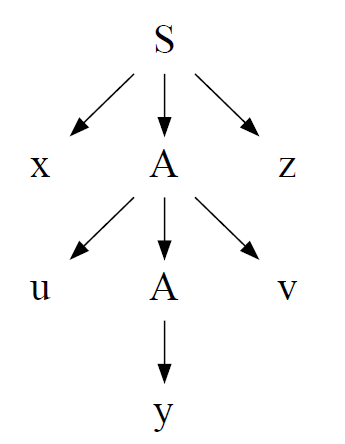
\includegraphics[scale=0.25]{images/2_14_1.png}
        \label{fig:first}
\end{figure}

Покажем, что $|uyv| \leq p = 2^{|N|}$. Пусть $|uyv| > p = 2^{|N|}$, тогда для дерева со стартом в $A$ можно сделать те же самые операции, значит, существует уровень, который больше $|N|$, значит, существует в поддереве пара $B \vdash B$, и $A$ -- не самый глубокий нетерминал.

Покажем, что $|uv| > 0$. Для любого нетерминального символа $C \in N$ верно, что $C$ не является $\varepsilon$-порождающим. Рассмотрим $D$ такой, что $D \vdash KA$ (за один шаг), $K \vdash r$, где $r$ — суффикс u, $|r| > 0$. Отсюда следует, что $|uv| \geq |u| \geq |r| > 0$. \EndProof

\par \Example Не КС-язык: $L=\{a^n b^n c^n\}$
\par $\blacktriangle$ Зафиксируем $p$ в лемме о разрастании. Рaссмотрим $w=a^p b^p c^p=xuyvz, |uv|>0, |uyv|\leq p$. Заметим, что в $uyv$ и $uv$ не может быть трех разных букв из $a,b,c$. Не умаляя общности $|uyv|_c=0, |uyv|_b>0$. Рассмотрим $k=2$: $$|w'|_b=|xu^2yv^2z|_b=|xuyvz|_b+|uv|_b>p$$ $$|xu^2yv^2z|_c=p+|uv|_c=p$$
\par Следовательно, $|w'|_b \neq |w'|_c$, а значит $w'$ не лежит в языке и выполнено отрицание леммы о разрастании, то есть язык не является КС $\blacksquare$
